%\documentclass[blue]{beamer}
%\usetheme{Boadilla}
% Class options include: notes, notesonly, handout, trans,
%                        hidesubsections, shadesubsections,
%                        inrow, blue, red, grey, brown
\documentclass[red]{beamer}


\mode<presentation> {
  \usetheme{Warsaw}
  \setbeamercovered{transparent}
}

% Theme for beamer presentation.
\usepackage{beamerthemesplit} 
\usepackage[czech]{babel}
\usepackage[utf8]{inputenc}
\usepackage[T1]{fontenc}
\usepackage{listings}

\title{Distribuovaný systém kontroly verzií - Git}    % Enter your title between curly braces
\author{Juraj Hreško}                 % Enter your name between curly braces
\institute{ecommerce.cz}      % Enter your institute name between curly braces
\date{\today}                    % Enter the date or \today between curly braces

\begin{document}

\begin{frame}
  \titlepage
\end{frame}


\section{Verzovacie systémy}



\begin{frame}
  \frametitle{Požiadavky na SCM}   % Insert frame title between curly braces
  \begin{itemize}
  \item ukladanie dát do archívu (repozitára)
\pause
  \item obnovenie dát z určitej doby
\pause
  \item porovnávanie verzií dát
\pause
  \item anotovanie dát
\pause
  \item riešenie prítupu viacerých vývojárov
\pause
 \item označovanie verzií špecifickým menom
\pause
 \item vetvenie vývoja
\pause
 \item zlučovanie vetví vývoja
  \end{itemize}
\end{frame}

\begin{frame}
  \frametitle{Typy verzovacích systémov}   % Insert frame title between curly braces
  \begin{itemize}
  \item "triviálne"
  \item centralizované (client-server)
  \item distribuované
  \end{itemize}
\end{frame}

\begin{frame}[fragile]
  \frametitle{"Triviálne"  verzovanie}   % Insert frame title between curly braces
   
  Použil už snáď každý pri zálohe napr. konfiguračných súborov. 

\begin{block}{Príklad}
\begin{verbatim}
    $ cp config.cfg config.old
    c:\>copy config.cfg config.old
\end{verbatim}
\end{block}
\pause
\begin{itemize}
\item vhodné pre jednu dostupnú "zálohu"
\item nesystematické pre viac súborov s históriou
\item nehovoriac o zdieľaní, vetvení a pod.
\end{itemize}

\end{frame}

\begin{frame}
  \frametitle{Centralizované systémy pre správu verzií}   % Insert frame title between curly braces

\begin{itemize}
\item architektúra typu klient-server
\item spoločný centrálny repozitár
\item vývoj prebieha v rámci pracovnej kópie
\item riešenie súčasného zápisu viacerých programátorov
\begin{itemize}
\item lock/modify/commit
\item modify/merge/commit
 \end{itemize}
\item zástupcovia: CVS, SVN, Perforce, TFS
 \end{itemize}
\end{frame}

\begin{frame}
  \frametitle{Distribuované systémy pre správu verzií}   % Insert frame title between curly braces

\begin{itemize}
\item neexistuje centrálny repozitár - každý je plnohodnotný
\item miesto operácie checkout operácia clone
\item repozitár == pracovná kópia
\item publikovanie zmien - vystavenie repozitára, push do vzdialenej vetvy, posielanie záplat e-mailom
 \end{itemize}
\end{frame}

\section{Výhody DSCM (Git)}

\begin{frame}
  \frametitle{Práca s lokálnym repozitárom}   % Insert frame title between curly braces

\begin{itemize}
\item neexistuje "jedno zraniteľné miesto" (single point of failure)
\item offline práca s repozitárom (vo vlaku, na chate, pri výpadku serverov)
\begin{itemize}
\item prechádzanie histórie
\item commity
\item vetvenie
 \end{itemize}
\item súkromie pri experimentoch
\item rýchlosť operácií
 \end{itemize}
\end{frame}

\begin{frame}
  \frametitle{Práca s repozitármi - schéma}

  \begin{figure}
  \centering
  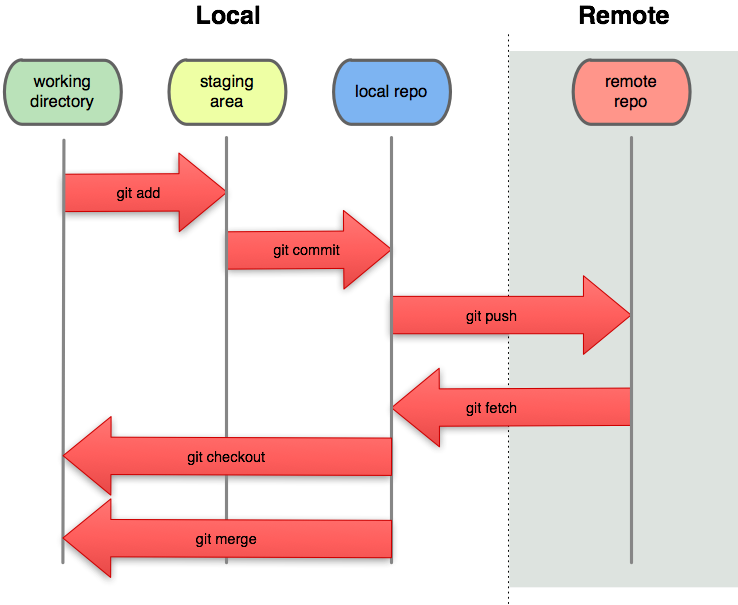
\includegraphics[scale=0.7]{git-pics/local-remote.png}
\end{figure}
\end{frame}

\subsection{Flexibilný workflow}
\begin{frame}
\frametitle{Flexibilný workflow}
\begin{itemize}
\item je možné pracovať s repozitármi rôznymi spôsobmi, v závislosti od druhu projektu
\item iné pre klasický centralizovaný vývoj, vlastné dokumenty, vývoj open source software
\item príklady niektorých možných workflow
\begin{itemize}
\item centralizovaný 
\item koordinátor
\item generál a pobočníci
 \end{itemize}
 \end{itemize}
\end{frame}

\begin{frame}
  \frametitle{Centralizovaný workflow}

  \begin{figure}
  \centering
  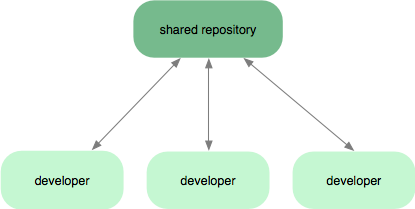
\includegraphics[scale=1]{git-pics/workflow-a.png}
\end{figure}
\end{frame}

\begin{frame}
  \frametitle{Workflow "koordinátor"}

  \begin{figure}
  \centering
  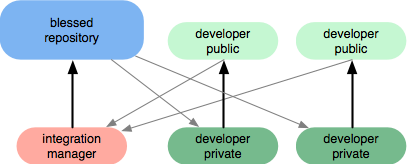
\includegraphics[scale=1]{git-pics/workflow-b.png}
\end{figure}
\end{frame}

\begin{frame}
  \frametitle{Workflow "generál a pobočníci"}

  \begin{figure}
  \centering
  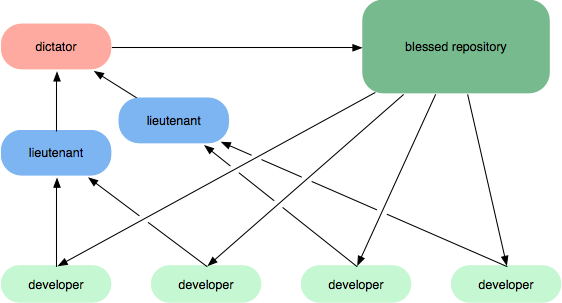
\includegraphics[scale=1]{git-pics/workflow-c.png}
\end{figure}
\end{frame}
	
\end{document}
